\documentclass[12pt]{article} % se puede cambiar por article
\usepackage{dtj_iteso}
\RequirePackage{amsmath,amsfonts,amssymb,amsthm}
\usepackage{eulervm} % tipografía con soporte para matemáticas
\usepackage{caption}
 
\usepackage{exercise}
\usepackage{graphicx}
% \DeclareMathOperator*{\argmax}{argmax}

% \newcommand{\vect}[1]{\boldsymbol{#1}}

\usepackage[utf8]{inputenc}
\usepackage[spanish,mexico]{babel}
% sgamex.sty from Rubinstein
\usepackage{sgamex}
\usepackage{forest}
\forestset{qtree/.style={for tree={parent anchor=south, 
           child anchor=north,align=center,inner sep=0pt}}}
          
\usepackage{setspace}
\onehalfspacing % doble espacio: \doublespacing

\title{Solución del Examen de la Unidad 2}
\author{Emmanuel Alcalá}
\date{\today}

\begin{document}
\maketitle

\begin{Exercise}[name={Respuesta}]

  \begin{enumerate}
    \setlength{\itemsep}{0pt}
    \setlength{\parskip}{0pt}
    \setlength{\parsep}{0pt}
    \item $ M_t = U(1+r)^t $ o si $ U=1 $, $ M_t = (1+r)^t $.
    \item $ u(t) = \sum_{t=1}^{\infty} \delta^{t-1}u^{(t)}$ con $ \delta = 1/(1+r)^t $.
  \end{enumerate}

\end{Exercise}

\begin{Exercise}[name={Respuesta}]

  \begin{enumerate}
    \setlength{\itemsep}{0pt}
    \setlength{\parskip}{0pt}
    \setlength{\parsep}{0pt}
    \item Tres subjuegos.
    \item ENPS $ = \{ (D,M),M \}$, con ganancias $ = (2, 0) $.
  \end{enumerate}

\end{Exercise}

\begin{Exercise}[name={Respuesta}]

  \begin{enumerate}
    \setlength{\itemsep}{0pt}
    \setlength{\parskip}{0pt}
    \setlength{\parsep}{0pt}
    \item Cuatro subjuegos.
    \item De información perfecta: todos los conjuntos de información son unitarios o, dicho de otra manera, los jugadores conocen el historial del juego cuando les toca mover.
    \item ENPS $ = \{ (ND,dr, bl),DR \}$, con ganancias $ = (10/3, 20/3) $. Conviene tomar la acción ND.
  \end{enumerate}

\end{Exercise}

\begin{Exercise}[name={Respuesta}]

  \begin{enumerate}
    \setlength{\itemsep}{0pt}
    \setlength{\parskip}{0pt}
    \setlength{\parsep}{0pt}
    \item ENPS $ = \{ (s, c, f),b\}$, con ganancias $ = (4, 4) $.
    \item Se convierte en árbol con información imperfecta:
          \begin{center}
            \begin{istgame}
              \xtdistance{15mm}{30mm}
              \istroot[-135](0)[initial node]<0>{J1}
              \istb{t}[a]{(3,5)}[l] \istb{s}[r] \endist
              \istroot(1)(0-2)<135>{J2}
              \istb{a}[al] \istb{b}[ar] \endist
              \xtdistance{10mm}{15mm}
              \istroot(2)(1-1)%<135>{J1}
              \istb{a}[al]{(2,2)} \istb{b}[ar]{(0,0)} \endist
              \istroot(3)(1-2)%<45>{J1}
              \istb{a}[al]{(1,1)} \istb{b}[ar]{(4,4)} \endist
              % \xtSubgameBox(1){(2-1)(3-2)}
              \xtInfoset(2)(3){J1}
            \end{istgame}
          \end{center}

          El segundo nodo, cuando mueve J2, es un subjuego que debe jugarse de forma simultánea. El ENPS se puede obtener con estrategias mixtas (1+ extra) o considerando dos escenarios. Nota: los resultados los doy considerando que cambiaron las acciones del jugador 1 a $ a, b $.\\
          $\text{ENPS}_1 = \{ (s, b),b\}$, con ganancias $ = (4, 4) $.\\
          $\text{ENPS}_2 = \{ (t, a),a\}$, con ganancias $ = (3, 5) $.
  \end{enumerate}

\end{Exercise}


\begin{Exercise}[name={Respuesta}]

  \begin{enumerate}
    \setlength{\itemsep}{0pt}
    \setlength{\parskip}{0pt}
    \setlength{\parsep}{0pt}
    \item El árbol es
          \begin{center}
            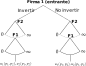
\includegraphics[width=0.6\textwidth]{figs/ex_p5_1.png}
          \end{center}
          Notar que tanto a la izquierda como a la derecha hay información imperfecta, por lo que se parece a un duopolio de Cournot, y se debe resolver de forma simultánea, a diferencia del duopoliode Stackelberg.
    \item Primero analizaré la segunda etapa. Cada firma escoge una $ p_i^* = \argmax_{p_i > 0} u_i(p_i, p_j) $.

          \textbf{Firma 1 invierte}: $ p_i^* = \argmax_{p_i > 0} u_i(p_i, p_j) = (1 - 2p_i + p_j)p_i $. La condición de primer orden, y despejando para $ p_i $ da
          \[p_i^* = \frac{1 + p_j}{4}\]
          para $ i = \{1, 2\}, i\neq j$ (es decir, usan estrategias simétricas).  Metiendo $ p_2^* $ en $ p_1^* $ nos da que $ p_1^* = 1/3$ (y lo mismo para el jugador 2), que son los precios en equilibrio. Las ganancias, sustituyendo $ p_1^* = 1/3 $ y $ p_2^* = 1/3 $ nos da $u_1(p_1, p_2) = \frac{2}{9} - I$ y $ u_2(p_1, p_2) = \frac{2}{9} $. Con $ I = 0.205 $, la utilidad es $u_1(p_1, p_2) = 0.017$.\\
          \textbf{Firma 1 no invierte}: en este caso, la firma 1 tiene un costo de $c$, por lo que su función es $ p_1^* = \argmax_{p_1 > 0} u_1(p_1, p_2; c) = (1 - 2p_1 + p_2)(p_1 - c) $, con $ c=1/2 $.La condición de primer orden resulta en
          \[p_1^* = \frac{2+p2}{4} \]
          Dado que la firma 2 no tiene costo, su función es la misma que cuando la firma 1 invierte, y que ya habíamos calculado $ p_2^* = \frac{1 + p_1}{4} $. Resolviendo para la firma 1, tenemos que el precio en equilibrio $ p_1^* $ es de $ 3/5 $, y para la firma 2 $ p_2^*  = 2/5$. La utilidad de la firma 1 cuando no invierte es

          \[
            u_1(p_1, p_2; c) = 1(-2*(3/5) + 2/5)(3/5 - 1/2) = 1/50 = 0.02
          \]
          Que es más que la utilidad cuando invierte (0.017). Por lo tanto, en equilibrio la firma 1 no invierte.
  \end{enumerate}

  \textbf{Extra}: La utilidad de no invertir es de $1/50$, la utilidad de unvertir es $ \frac{2}{9} -I \geq 0.02$, despejando para $ I $ nos da $ I \leq 0.202\bar 2$.

\end{Exercise}
\end{document}